\documentclass{beamer}

\usetheme{CambridgeUS}
\usecolortheme{orchid}

\usepackage[utf8]{inputenc}
\usepackage[T1]{fontenc}

% Paths
\newcommand{\figs}{../figs}
\newcommand{\data}{../data}
\newcommand{\code}{../code}

% URL styles
\usepackage{url}
\urlstyle{sf}

% Units
\usepackage[detect-weight=true, binary-units=true]{siunitx}
\DeclareSIUnit\flop{Flops}

% Math
\usepackage{amsmath}
\usepackage{amssymb}
\usepackage{bm}
\usepackage{nicefrac}
\newcommand{\dif}[1]{{\;\text{d}#1}}

% Graphics
\usepackage{graphicx}
\usepackage{caption}
\usepackage{subcaption}
\graphicspath{{../figs/}}

% Tikz
\usepackage{tikz}
\usetikzlibrary{positioning,shapes,arrows,calc,intersections}
\usepackage{pgfplots}
\usepgfplotslibrary{dateplot}
\pgfplotsset{compat=1.8}

% Colors
\definecolor{darkblue}{HTML}{00688B}
\definecolor{darkgreen}{HTML}{6E8B3D}
\definecolor{cadet}{HTML}{DAE1FF}
\definecolor{salmon}{HTML}{FFB08A}

% Listings
\usepackage{textcomp}
\usepackage{listings}
\lstset{
  keywordstyle=\bfseries\color{orange},
  stringstyle=\color{darkblue!80},
  commentstyle=\color{darkblue!80},
  showstringspaces=false,
  basicstyle=\ttfamily,
  upquote=true,
}
\lstdefinestyle{fortran}{
  language=Fortran,
  morekeywords={for},
  deletekeywords={status},
}
\lstdefinestyle{c}{
  language=C,
  morekeywords={include},
}
\lstdefinestyle{glsl}{
  language=C,
  morekeywords={attribute, vec2, vec3, vec4, varying, uniform, mat2, mat3, mat4},
}
\lstdefinestyle{cuda}{
  language=C,
  morekeywords={__global__, __device__, __host__},
}
\lstdefinestyle{shell}{
  language=bash,
  morekeywords={mkdir, ssh, cmake},
}

% Double hlines
\usepackage{hhline}

% Misc
\usepackage{nth}

\subtitle{TMA4280---Introduction to Supercomputing}

\begin{document}


\title{Iterative Poisson solvers}
\author{Eivind Fonn}
\institute{SINTEF ICT / NTNU}
\date{December 2015}
\maketitle

\begin{frame}
  \frametitle{Iterative solves}
  \begin{itemize}
  \item So far we have considered direct methods, which work on the matrix and
    its elements.
  \item Now: iterative methods, which seek to solve the system by iteration,
    gradually improving an estimate of the solution.
  \item In general they only yield an approximation to the solution, instead of
    the exact solution.
  \item Important concept: the \emph{residual}
    \[
      \bm r = \bm b - \bm A \bm x^k
    \]
    at some iteration $k$.
  \item Obviously if $\bm x$ is the exact solution then $\bm r = \bm 0$.
  \item The residual is used as a ``forward'' error estimate, but should not be
    confused with the actual error.
  \end{itemize}
\end{frame}

\begin{frame}
  \frametitle{Fixed point iteration}
  \begin{itemize}
  \item It's tempting to try some schemes we learned in elementary calculus.
  \item Rewrite the problem on the form $\bm x =g(\bm x)$ for some function $g$:
    \[
      \bm A \bm x = \bm b \Rightarrow (\bm A + \bm I) \bm x - \bm b = \bm x,
    \]
    thus
    \[
      \bm x^{k+1} = g(\bm x^k) = (\bm A + \bm I) \bm x^k - \bm b.
    \]
  \item Unfortunately this only works if $\bm g$ is a \emph{contraction}, which
    means that
    \[
      \max_i |\lambda_i(\bm A + \bm I)| < 1
    \]
    which is seldom the case.
  \end{itemize}
\end{frame}

\begin{frame}
  \frametitle{Newton iteration}
  \begin{itemize}
  \item Newton iteration works on a problem on the form $f(\bm x) = 0$, in other
    words $f(\bm x) = \bm A \bm x - \bm b$.
  \item It takes the form
    \[
      \bm x^{k+1} = \bm x^k - \bm Df(\bm x^k)^{-1} f(\bm x^k)
    \]
    where $\bm Df$ is the derivative (Jacobian) matrix of $f$.
  \item In our case we get $\bm Df = \bm A$ so
    \[
      \bm x^{k+1} = \bm x^k - \bm A^{-1}(\bm A \bm x^{k} - \bm b) = \bm A^{-1} \bm b
    \]
    so we are back to square one.
  \end{itemize}
\end{frame}

\begin{frame}
  \frametitle{Splitting methods}
  \begin{itemize}
  \item Split the matrix $\bm A$ into three parts,
    \[
      \underbrace{
        \begin{pmatrix}
          \\
          a_{21} \\
          a_{31} & a_{32} \\
          \vdots & \vdots & \ddots
        \end{pmatrix}
      }_{\bm L}
      +
      \underbrace{
        \begin{pmatrix}
          a_{11} \\
          & a_{22} \\
          && a_{33} \\
          &&& \ddots
        \end{pmatrix}
      }_{\bm D}
      +
      \underbrace{
        \begin{pmatrix}
          & a_{12} & a_{13} & \cdots \\
          && a_{23} & \cdots \\
          &&& \ddots
        \end{pmatrix}
      }_{\bm U}
    \]
  \item Not to be confused with $\bm L$ and $\bm U$ from LU decomposition.
  \end{itemize}
\end{frame}

\begin{frame}
  \frametitle{Gauss-Jacobi}
  \begin{itemize}
  \item Reorganize the system
    \begin{align*}
      \bm A \bm x &= \bm b \\
      (\bm L + \bm D + \bm U) \bm x &= \bm b \\
      \bm D \bm x &= \bm b - (\bm L + \bm U) \bm x
    \end{align*}
  \item And form an iterative scheme:
    \[
      \bm D \bm x^{k+1} = \bm b - (\bm L + \bm U) \bm x^k.
    \]
  \item This is the \emph{Gauss-Jacobi} method.
  \end{itemize}
\end{frame}

\begin{frame}
  \frametitle{Gauss-Seidel}
  \begin{itemize}
  \item Likewise, we can do
    \begin{align*}
      \bm A \bm x &= \bm b \\
      (\bm L + \bm D + \bm U) \bm x &= \bm b \\
      (\bm L + \bm D) \bm x &= \bm b - \bm U \bm x
    \end{align*}
  \item And form an iterative scheme:
    \[
      (\bm L + \bm D) \bm x^{k+1} = \bm b - \bm U \bm x^k.
    \]
  \item This is the \emph{Gauss-Seidel} method.
  \end{itemize}
\end{frame}

\begin{frame}
  \frametitle{Splitting methods}
  \begin{itemize}
  \item The rationales behind these methods are easy to spot on component form.
  \item Gauss-Jacobi solves the $i$th equation for the $i$th unknown, given the
    previous approximate values of the other unknowns:
    \[
      x_i^{k+1} = \frac{1}{a_{ii}}\left( b_i - \sum_{j \not= i} a_{ij} x_j^k \right)
    \]
  \item Gauss-Seidel does the same, but uses ``updated'' values when available.
    \[
      x_i^{k+1} = \frac{1}{a_{ii}}
      \left( b_i - \sum_{j=1}^{i-1} a_{ij} x_j^{k+1} - \sum_{j=i+1}^{N} a_{ij} x_j^k \right)
    \]
  \end{itemize}
\end{frame}

\begin{frame}[fragile]
  \frametitle{Gauss-Jacobi}
\begin{lstlisting}[style=c, basicstyle=\ttfamily\scriptsize]
void GaussJacobi(Matrix A, Vector u, int maxit) {
  int it=0, i, j;
  Vector b, e = vector(u->len);  // initialize both
  copy(b, u); fill(u, 0.0);
  while (it++ < maxit) {
    copy(e, u); copy(u, b);
    for (i = 0; i < A->rows; ++i) {
      for (j = 0; j < A->cols; ++j) {
        if (j != i)
          u[i] -= A[j][i] * e[j];
      }
      u[i] /= A[i][i];
    }
  }
  free(b); free(e);
}
\end{lstlisting}
\end{frame}

\begin{frame}[fragile]
  \frametitle{Gauss-Jacobi with residual tolerance}
\begin{lstlisting}[style=c, basicstyle=\ttfamily\scriptsize]
void GaussJacobi(Matrix A, Vector u, double tol, int maxit) {
  int it=0, i, j;
  Vector b, e, r = vector(u->len);  // initialize all
  copy(b, u); fill(u, 0.0);
  double rl = infnorm(b), norm = inf;
  while (it++ < maxit && norm > tol * rl) {
    copy(e, u); copy(u, b);
    for (i = 0; i < A->rows; ++i) {
      for (j = 0; j < A->cols; ++j) {
        if (j != i)
          u[i] -= A[j][i] * e[j];
      }
      r[i] = u[i] - A[i][i] * e[i];
      u[i] /= A[i][i];
    }
    norm = infnorm(r);
  }
  free(b, e, r);
}
\end{lstlisting}
\end{frame}

\begin{frame}[fragile]
  \frametitle{Gauss-Seidel}
\begin{lstlisting}[style=c, basicstyle=\ttfamily\scriptsize]
void GaussSeidel(Matrix A, Vector u, int maxit) {
  int it=0, i, j;
  Vector b, e = vector(u->len);  // initialize both
  copy(b, u); fill(u, 0.0);
  while (it++ < maxit) {
    copy(e, u); copy(u, b);
    for (i = 0; i < A->rows; ++i) {
      for (j = 0; j < A->cols; ++j) {
        if (j != i)
          u[i] -= A[j][i] * e[j];
      }
      u[i] /= A[i][i]; e[i] = u[i];
    }
  }
  free(b, e);
}
\end{lstlisting}
\end{frame}

\begin{frame}[fragile]
  \frametitle{Gauss-Seidel with residual tolerance}
\begin{lstlisting}[style=c, basicstyle=\ttfamily\scriptsize]
void GaussSeidel(Matrix A, Vector u, double tol, int maxit) {
  int it=0, i, j;
  Vector b, e, r = vector(u->len);  // initialize all
  copy(b, u); fill(u, 0.0);
  double rl = infnorm(b), norm = inf;
  while (it++ < maxit && norm > tol * rl) {
    copy(e, u); copy(u, b);
    for (i = 0; i < A->rows; ++i) {
      for (j = 0; j < A->cols; ++j) {
        if (j != i)
          u[i] -= A[j][i] * e[j];
      }
      r[i] = u[i] - A[i][i] * e[i];
      u[i] /= A[i][i]; e[i] = u[i];
    }
    norm = infnorm(r);
  }
  free(b, e, r);
}
\end{lstlisting}
\end{frame}

\begin{frame}[fragile]
  \frametitle{Gauss-Jacobi parallelized}
  \begin{itemize}
  \item Gauss-Jacobi iterations are easily parallelized.
  \item With OpenMP, for example, we can just fork on the rows.
\begin{lstlisting}[style=c, basicstyle=\ttfamily\footnotesize]
    // ...
    #pragma omp parallel for schedule(static)
    for (i = 0; i < A->rows; ++i) {
      for (j = 0; j < A->cols; ++j) {
        if (j != i)
          u[i] -= A[j][i] * e[j];
      }
      u[i] /= A[i][i];
    }
    // ...
\end{lstlisting}
  \end{itemize}
\end{frame}

\begin{frame}[fragile]
  \frametitle{Matrix-free iterations}
  \begin{itemize}
  \item A characteristic property of iterative methods is that, unlike direct
    methods, there is usually no need to explicitly store the matrix.
  \item Usually they work just fine if you have a function for calculating the
    matrix-vector product, or (in case of the splitting methods) a function for
    updating a single unknown.
  \item This allows us to heavily optimize Gauss-Jacobi.
\begin{lstlisting}[style=c, basicstyle=\ttfamily\footnotesize]
    // ...
    #pragma omp parallel for schedule(static)
    for (i = 0; i < A->rows; ++i) {
      if (i > 0)
        u[i] += e[i-1];
      if (i < e->len - 1)
        u[i] += e[i+1];
      u[i] /= 2.0;
    }
    // ...
\end{lstlisting}
  \end{itemize}
\end{frame}

\begin{frame}
  \frametitle{Gauss-Seidel parallelized}
  \begin{itemize}
  \item The Gauss-Seidel method is more difficult to parallelize.
  \item Since the data from one iteration is immediately required in the next,
    there is no way to implement Gauss-Seidel as given in a parallel manner.
  \item We can do something similar, however. There is nothing that mandates we
    sweep the unknowns in a specific order.
  \item If we change the order, we can do better.
  \end{itemize}
\end{frame}

\begin{frame}
  \frametitle{Gauss-Seidel parallelized}
  \begin{center}
    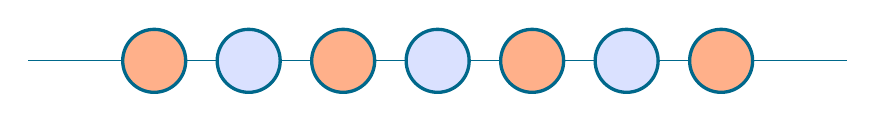
\begin{tikzpicture}[scale=0.4]
      \draw[darkblue] (-13,0) -- (13,0);
      \draw[darkblue, fill=salmon, very thick] (-9,0) circle (1);
      \draw[darkblue, fill=cadet, very thick] (-6,0) circle (1);
      \draw[darkblue, fill=salmon, very thick] (-3,0) circle (1);
      \draw[darkblue, fill=cadet, very thick] (0,0) circle (1);
      \draw[darkblue, fill=salmon, very thick] (3,0) circle (1);
      \draw[darkblue, fill=cadet, very thick] (6,0) circle (1);
      \draw[darkblue, fill=salmon, very thick] (9,0) circle (1);
    \end{tikzpicture}
  \end{center}
  \begin{itemize}
  \item By ``coloring'' the nodes in an alternating pattern, we see that ``red''
    nodes only couple to ``blue'' ones, and vice versa.
  \item We can sweep all red nodes in parallel, and then sweep all blue nodes in
    parallel.
  \item Note: this is not the same as Gauss-Seidel, not even mathematically.
  \end{itemize}
\end{frame}

\begin{frame}[fragile]
  \frametitle{Gauss-Seidel parallelized}
\begin{lstlisting}[style=c, basicstyle=\ttfamily\footnotesize]
  for (j = 0; j < 2; ++j) {
    // ...
    #pragma omp parallel for schedule(static)
    for (i = j; i < e->len; i += 2) {
      if (i > 0)
        u[i] += e[i-1];
      if (i < e->len - 1)
        u[i] += e[i+1];
      u[i] /= 2.0; e[i] = u[i];
    }
    // ...
  }
\end{lstlisting}
\end{frame}

\begin{frame}[fragile]
  \frametitle{Redundant storage}
  \begin{itemize}
  \item Another freedom offered by iterative schemes is that we can store data
    as we see fit.
  \item For the direct methods, we eliminated the nodes on the boundary, since
    they are not part of the system.
  \item In iterative methods, we are free to explicitly store the boundary
    elements.
  \item This is very beneficial, in particular when we consider MPI
    parallelization (soon).
  \end{itemize}
\end{frame}

\begin{frame}[fragile]
  \frametitle{Gauss-Jacobi with redundant storage}
\begin{lstlisting}[style=c, basicstyle=\ttfamily\footnotesize]
    // ...
    #pragma omp parallel for schedule(static)
    for (i = 1; i < e->len - 1; ++i) {
      u[i] += e[i-1];
      u[i] += e[i+1];
      u[i] /= 2.0;
    }
    // ...
\end{lstlisting}
\end{frame}

\begin{frame}
  \frametitle{Gauss Jacobi with MPI}
  \begin{itemize}
  \item There are essentially two ways to partition a linear system of equations
    \begin{enumerate}
    \item We can partition the data structure (the matrix and vector)
    \item We can partition the problem that generated the linear system in the
      first place. This is referred to as \emph{domain decompoisition}.
    \end{enumerate}
  \item These approaches are not independent. In particular, domain
    decomposition can be seen as a way of generating the data structure
    partitioning. (More on this later.)
  \end{itemize}
\end{frame}

\begin{frame}
  \frametitle{Matrix partitioning}
  Row-based division
  \[
    \begin{pmatrix}
      \cdots & \bm A_0 & \cdots \\
      \cdots & \bm A_1 & \cdots \\
      \cdots & \bm A_2 & \cdots
    \end{pmatrix}
    \begin{pmatrix}
      \bm x_0 \\ \bm x_1 \\ \bm x_2
    \end{pmatrix}
    =
    \begin{pmatrix}
      \bm b_0 \\ \bm b_1 \\ \bm b_2
    \end{pmatrix}
  \]
  Process $p$ can evaluate in two steps:
  \begin{enumerate}
  \item Collect (reduce) the entire vector $\bm x$
  \item Perform the local product $\bm A_p \bm x$
  \end{enumerate}
\end{frame}

\begin{frame}
  \frametitle{Matrix partitioning}
  Column-based division
  \[
    \begin{pmatrix}
      \vdots & \vdots & \vdots \\
      \bm A_0 & \bm A_1 & \bm A_2 \\
      \vdots & \vdots & \vdots
    \end{pmatrix}
    \begin{pmatrix}
      \bm x_0 \\ \bm x_1 \\ \bm x_2
    \end{pmatrix}
    =
    \begin{pmatrix}
      \bm b_0 \\ \bm b_1 \\ \bm b_2
    \end{pmatrix}
  \]
  Process $p$ can evaluate in two steps:
  \begin{enumerate}
  \item Perform the local product $\bm A_p \bm x_p$
  \item Distribute (reduce) the entire vector $\bm x$
  \end{enumerate}
\end{frame}

\begin{frame}
  \frametitle{Domain decomposition}
  \begin{itemize}
  \item Common to both these approaches is that we need to exchange the entire
    vector for each multiplication.
  \item Domain decomposition can help reduce the amount of communication
    necessary.
  \item Essentially, it highlights a nearly block-diagonal matrix structure.
  \item Can be used for all kinds of grids.
  \end{itemize}
  \begin{center}
    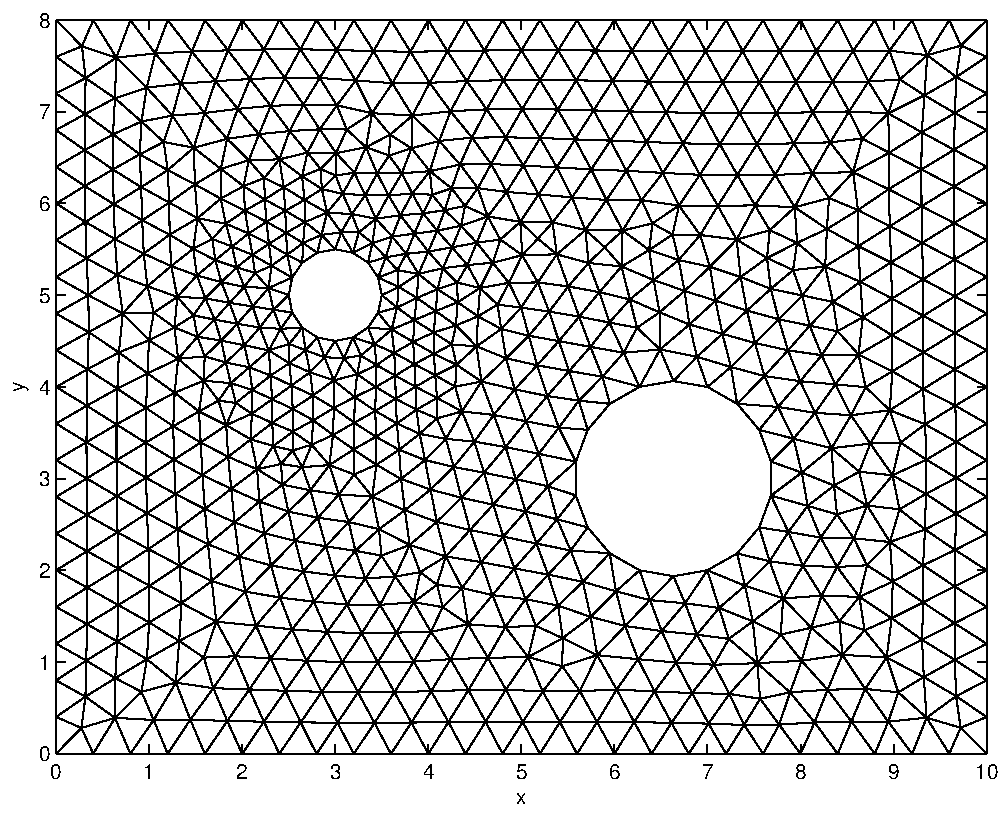
\includegraphics[height=3.5cm]{\figs/grid2D_1domain}
    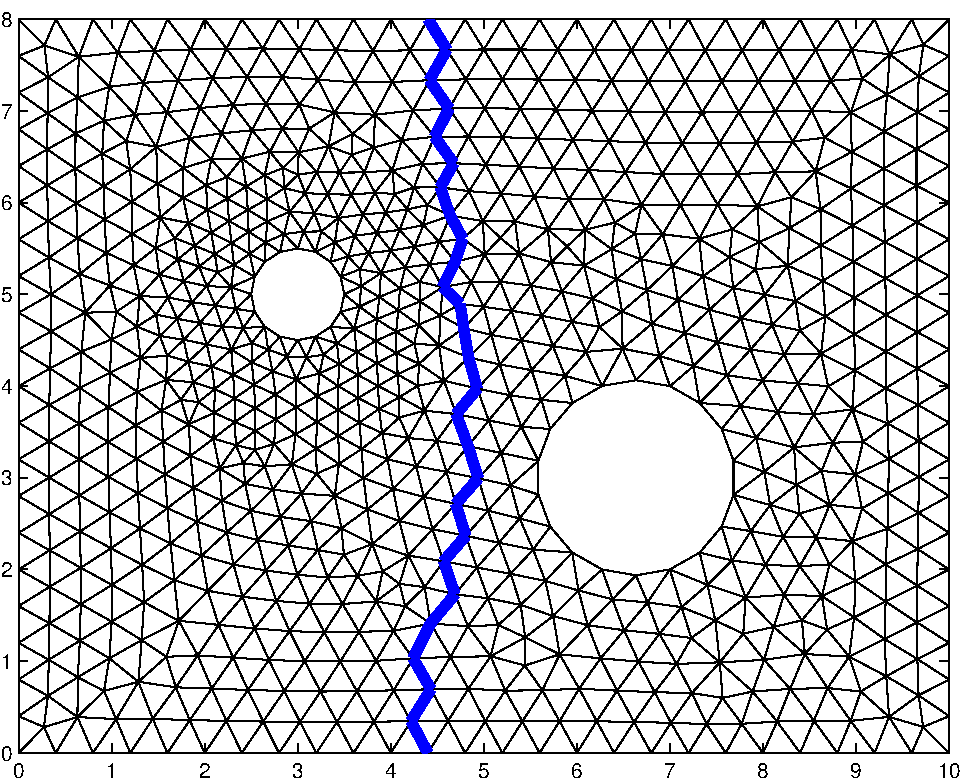
\includegraphics[height=3.5cm]{\figs/grid2D_2domains}
  \end{center}
\end{frame}

\begin{frame}
  \frametitle{Gauss-Jacobi with MPI (1D)}
  \begin{itemize}
  \item We partition the mesh. In 1D this is the same as splitting a vector.
    \begin{align*}
      P_0: &\qquad \begin{pmatrix} x_1 & x_2 & \cdots & x_q \end{pmatrix} \\
      P_1: &\qquad \begin{pmatrix} x_{q+1} & x_{q+2} & \cdots & x_{2q} \end{pmatrix} \\
      \vdots &
    \end{align*}
  \item On each process, use a redundant storage format, with extra elements at
    the start and end of the vector. Even on ``interior'' processes.
    \begin{align*}
      P_0: &\qquad \begin{pmatrix}
        {\color{gray} x_0} & x_1 & x_2 & \cdots & x_q & {\color{gray} x_{q+1}}
      \end{pmatrix} \\
      P_1: &\qquad \begin{pmatrix}
        {\color{gray} x_q} & x_{q+1} & x_{q+2} & \cdots & x_{2q} & {\color{gray} x_{2q+1}}
      \end{pmatrix} \\
      \vdots &
    \end{align*}
  \end{itemize}
\end{frame}

\begin{frame}
  \frametitle{Gauss-Jacobi with MPI (1D)}
  \begin{itemize}
  \item The only difference required now is to obtain the neighbouring boundary
    values from the next and previous process before the Gauss-Jacobi iteration.
  \item MPI has built-in functions for setting up processes in a
    \emph{topology}. This is easy to do manually in one dimension but they are
    very handy in several dimensions:
    \begin{itemize}
    \item \texttt{MPI\_Dims\_create}
    \item \texttt{MPI\_Cart\_create}
    \item \texttt{MPI\_Cart\_coords}
    \item \texttt{MPI\_Cart\_Shift}
    \item \texttt{MPI\_Sendrecv}
    \end{itemize}
  \end{itemize}
\end{frame}

\begin{frame}
  \frametitle{Gauss-Jacobi with MPI (2D)}
  \begin{itemize}
  \item For convenience, we store our solution in a matrix.
  \item We want to partition it. Several possibilities:
    \[
      \begin{pmatrix}
        \vdots & \vdots & \vdots & \vdots \\
        \bm X_0 & \bm X_1 & \bm X_2 & \bm X_3 \\
        \vdots & \vdots & \vdots & \vdots
      \end{pmatrix}
      \quad
      \begin{pmatrix}
        \bm X_0 & \bm X_1 \\
        \bm X_2 & \bm X_3
      \end{pmatrix}
      \quad
      \begin{pmatrix}
        \cdots & \bm X_0 & \cdots \\
        \cdots & \bm X_1 & \cdots \\
        \cdots & \bm X_2 & \cdots \\
        \cdots & \bm X_3 & \cdots
      \end{pmatrix}
    \]
  \item The MPI tools allow us to handle all these cases with essentially the
    same code.
  \end{itemize}
\end{frame}

\begin{frame}
  \frametitle{Distributed arrays}
  \begin{itemize}
  \item Such arrays are called \emph{darrays}---distrbuted arrays.
  \item The functionality is heavily inspired by the \emph{High Performance
      Fortran} standard.
  \item The term \emph{topology} means, in laymans terms, ``how stuff is
    connected.''
  \item An array partitioning consists of a topology and a mapping of processes
    onto this topology.
  \end{itemize}
\end{frame}

\begin{frame}
  \frametitle{Distributed arrays}
  An example topology.
  \begin{center}
    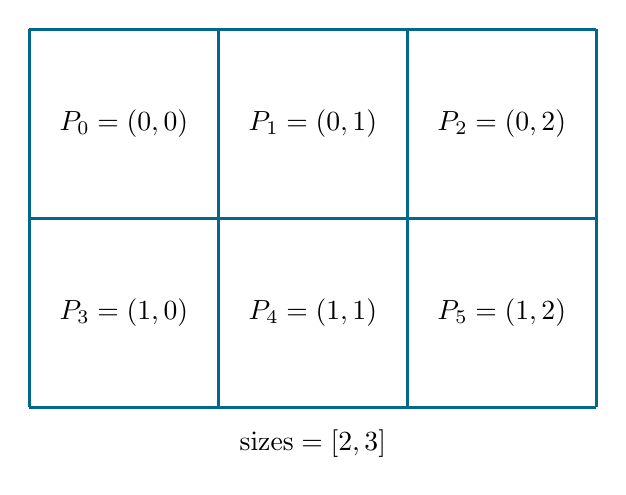
\begin{tikzpicture}[scale=0.8]
      \foreach \i in {0,3,6,9} {
        \draw[darkblue, very thick] (\i,0) -- (\i,6);
      }
      \foreach \i in {0,3,6} {
        \draw[darkblue, very thick] (0,\i) -- (9,\i);
      }
      \node at (1.5,4.5) {$P_0 = (0,0)$};
      \node at (4.5,4.5) {$P_1 = (0,1)$};
      \node at (7.5,4.5) {$P_2 = (0,2)$};
      \node at (1.5,1.5) {$P_3 = (1,0)$};
      \node at (4.5,1.5) {$P_4 = (1,1)$};
      \node at (7.5,1.5) {$P_5 = (1,2)$};
      \node[anchor=north] at (4.5,-0.2) {$\text{sizes} = [2,3]$};
    \end{tikzpicture}
  \end{center}
\end{frame}

\begin{frame}
  \frametitle{Distributed arrays}
  \begin{itemize}
  \item Here: a Cartesian topology expressed as the number of processes along
    each dimension ($2$ and $3$, respectively).
  \item The location of a particular domain in the topology can be expressed as
    an integer along each dimension.
  \item A mapping of the processes onto the topology (e.g. $P_1 \leftrightarrow
    (0,1)$).
  \end{itemize}
\end{frame}

\begin{frame}[fragile]
  \frametitle{Distributed arrays}
  \begin{itemize}
  \item \texttt{MPI\_Dims\_create} assigns sizes to each dimension.
  \item Block partitioning
\begin{lstlisting}[style=c]
  int sizes[2];
  sizes[0] = sizes[1] = 0;
  MPI_Dims_create(size, 2, sizes);
\end{lstlisting}
  \item Strip partitioning: specify a dimension by setting it to a nonzero
    value.
\begin{lstlisting}[style=c]
  int sizes[2];
  sizes[0] = 1; sizes[1] = 0;
  MPI_Dims_create(size, 2, sizes);
\end{lstlisting}
  \item Upon return the \texttt{sizes} array holds the size of each dimension.
  \end{itemize}
\end{frame}

\begin{frame}[fragile]
  \frametitle{Distributed arrays}
  \begin{itemize}
  \item To generate the mapping, we have to define a new communicator with the
    topology attached to it.
\begin{lstlisting}[style=c]
  int periodic[2];
  periodic[0] = periodic[1] = 0;
  MPI_Cart_create(MPI_COMM_WORLD, 2, sizes,
                  periodic, 0, &new_comm);
\end{lstlisting}
  \item The function can optionally reorder the processes (give them new ranks)
    and handle periodic topologies.
  \item The new communicator is stored in \texttt{new\_comm}.
  \end{itemize}
\end{frame}

\begin{frame}[fragile]
  \frametitle{Distributed arrays}
  \begin{itemize}
  \item Each process can now query for their precise coordinates using the
    \texttt{MPI\_Cart\_coords} function.
\begin{lstlisting}[style=c]
  int coords[2];
  MPI_Cart_coords(new_comm, rank, 2, coords);
\end{lstlisting}
  \item Note that unless you specified no reordering, the process may have a
    different rank in the new communicator than in the old one!
  \end{itemize}
\end{frame}

\begin{frame}[fragile]
  \frametitle{Distributed arrays}
  \begin{itemize}
  \item To send data a certain number of steps in one direction, use
    \texttt{MPI\_Cart\_shift} to compute, for any given process, the process to
    send to and the one to receive from.
\begin{lstlisting}[style=c]
  int send_to, receive_from;
  MPI_Cart_shift(new_comm, 1, 1,
                 &receive_from, &send_to);
\end{lstlisting}
  \item The function may give you the value \texttt{MPI\_PROC\_NULL} for
    processes near the boundary, which is safe to pass to other message
    functions and which results effectively in a effective no-op.
  \item You can use \texttt{MPI\_Sendrecv} to simultaneously send and receive to
    and from two different processes.
  \end{itemize}
\end{frame}

\end{document}

